\documentclass{standalone}
\usepackage{pgfplots}
\pgfplotsset{width=10cm, compat=1.18}
\usetikzlibrary{patterns}


\begin{document}
		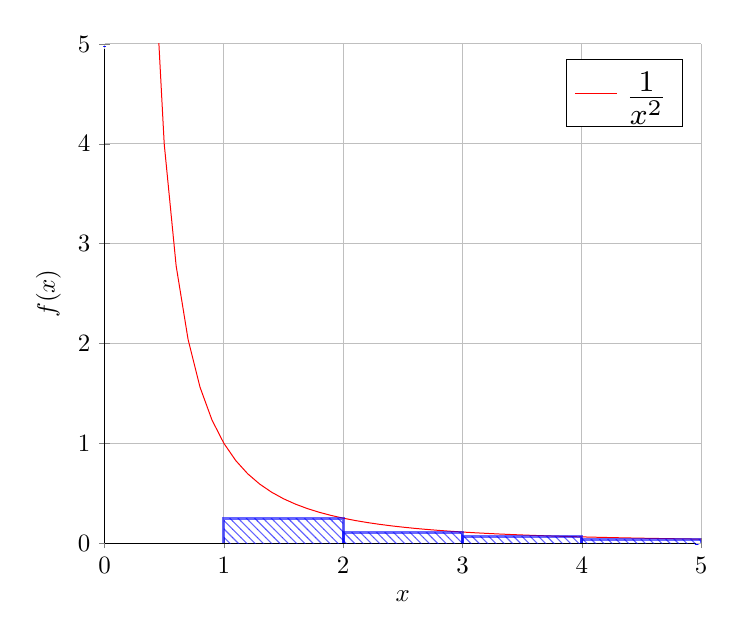
\begin{tikzpicture}[scale=0.9]
			\begin{axis}[
				axis lines=left,
				xlabel=$x$,
				ylabel=$f(x)$,
				xmin=0, xmax=5,
				ymin=0, ymax=5,
				grid=major,
				legend pos=north east,
				legend style={font=\large, scale=1.5, nodes={scale=1.5}},
				pattern color=blue, 
				pattern=horizontal lines
				]
				\addplot[
				domain=0.1:5,
				samples=50,
				color=red
				] {1/x^2};
				\addlegendentry{$\frac{1}{x^2}$}
				
				\draw[blue, very thick, opacity=0.6] (axis cs: 1,0) -- (axis cs: 1,{1/2^2}) -- (axis cs: 2,{1/2^2}) -- (axis cs: 2,0);
				\draw[blue, very thick, opacity=0.6] (axis cs: 2,0) -- (axis cs: 2,{1/3^2}) -- (axis cs: 3,{1/3^2}) -- (axis cs: 3,0);
				\draw[blue, very thick, opacity=0.6] (axis cs: 3,0) -- (axis cs: 3,{1/4^2}) -- (axis cs: 4,{1/4^2}) -- (axis cs: 4,0);
				\draw[blue, very thick, opacity=0.6] (axis cs: 4,0) -- (axis cs: 4,{1/5^2}) -- (axis cs: 5,{1/5^2}) -- (axis cs: 5,0);
				\fill[pattern=north west lines, pattern color=blue, opacity=0.6] 
				(axis cs: 1,0) rectangle (axis cs: 2,{1/2^2});
				\fill[pattern=north west lines, pattern color=blue, opacity=0.6] 
				(axis cs: 2,0) rectangle (axis cs: 3,{1/3^2});
				\fill[pattern=north west lines, pattern color=blue, opacity=0.6] 
				(axis cs: 3,0) rectangle (axis cs: 4,{1/4^2});
				\fill[pattern=north west lines, pattern color=blue, opacity=0.6] 
				(axis cs: 4,0) rectangle (axis cs: 5,{1/5^2});
			\end{axis}
		\end{tikzpicture}
\end{document}